\documentclass[11pt,a4paper,oneside]{article}
\usepackage[latin1]{inputenc}
\usepackage{amsmath}
\usepackage{amsfonts}
\usepackage{amssymb}
\usepackage{graphicx}
\usepackage{color}
\usepackage {tikz}
\usepackage{fancyvrb}
\usepackage{multicol}
\usepackage{caption}
\usepackage{subfig}
\usetikzlibrary {er}
\usepackage[left=2.00cm, right=2.00cm, top=1.00cm]{geometry}
\graphicspath{{./}}
\fvset{tabsize=4}

\begin{document}
	\title{DS 294 - Data Analysis and Visualization - Assignment 3}
	\author{Shriram R. \\ M Tech (CDS) \\ 06-02-01-10-51-18-1-15763}
	\maketitle	
	
	\section{Introduction}
	A 3D volume was sampled and visualized as contours and as surface in this assignment. The following section covers the description, screenshots and code. Code has been written in Python due to installation issues of Tcl version.
	
	\section{Description}
	
	The code uses vtkSampleFunction() to define the sampling volume to specfied range. A volume of interest which $z=15$ plane is extracted through vtkExtractVOI() function. There are two Actors: Outline which is in black color and Contour/Image at $z = 15$. Only outline can be shown by just removing the other actor from the window.
	
	\subsection{Contour}
	Contours are drawn at $z = 15$ using vtkContourFilter() with the specified no. of contours and range. The contours are mapped using vtkPolyDataMapper() with the given scalar range.
	
	\subsection{Image}
	The $z=15$ is also viewed as an image by mapping the values through a lookup table created with vtkLookupTable() with specified range ($0.0, 1.2$). The table and image are combined with vtkImageMapToColors() and rendered through vtkImageActor().
	
	\section{Screenshot}	
		
	\begin{center}
		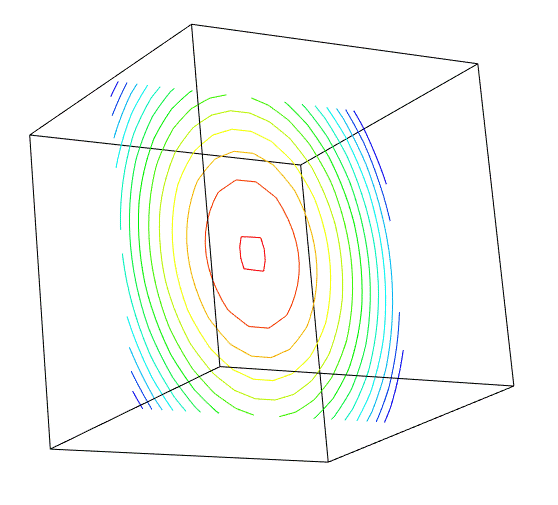
\includegraphics[scale=0.4]{1.png}	\\
		With Contour	
	\end{center}

    \begin{center}
    	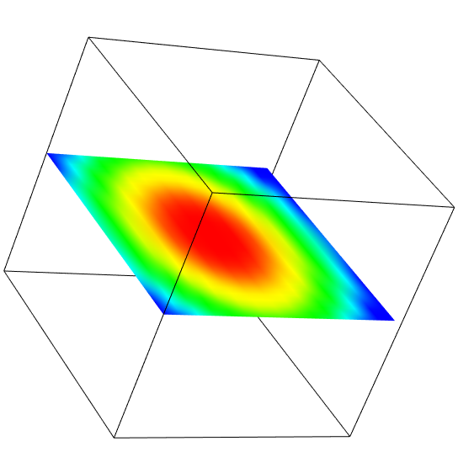
\includegraphics[scale=0.5]{3.png} \\
    	Without Contour (Image Rendering)	
    \end{center}

    \begin{center}
    	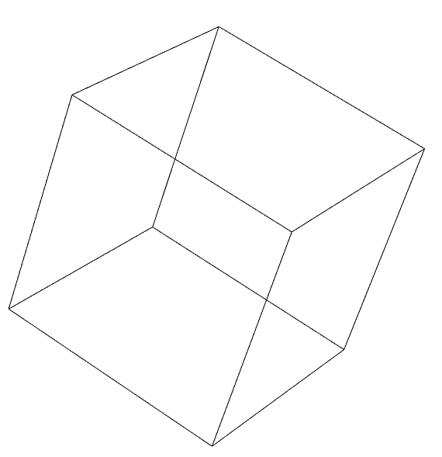
\includegraphics[scale=0.5]{2.png} \\
    	Only Outline	
    \end{center}

    \section{Code - Contours - Python}
    \begin{verbatim}
    #!/usr/bin/env python
   
    import vtk
    
    # Quadric definition.
    quadric = vtk.vtkQuadric()
    quadric.SetCoefficients(.5, 1, .2, 0, .1, 0, 0, .2, 0, 0)
    
    # The vtkSampleFunction uses the quadric function and evaluates function
    # value over a regular lattice (i.e., a volume).
    sample = vtk.vtkSampleFunction()
    sample.SetSampleDimensions(30, 30, 30)
    sample.SetImplicitFunction(quadric)
    sample.ComputeNormalsOff()
    sample.Update()
    
    # Here a single slice (i.e., image) is extracted from the volume.
    extract = vtk.vtkExtractVOI()
    extract.SetInputConnection(sample.GetOutputPort())
    extract.SetVOI(0, 29, 0, 29, 15, 15)
    extract.SetSampleRate(1, 2, 3)
    
    # The image is contoured to produce contour lines. Thirteen contour values
    # ranging from (0,1.2) inclusive are produced.
    contours = vtk.vtkContourFilter()
    contours.SetInputConnection(extract.GetOutputPort())
    contours.GenerateValues(13, 0.0, 1.2)
    
    # The contour lines are mapped to the graphics library.
    contMapper = vtk.vtkPolyDataMapper()
    contMapper.SetInputConnection(contours.GetOutputPort())
    contMapper.SetScalarRange(0.0, 1.2)
    
    contActor = vtk.vtkActor()
    contActor.SetMapper(contMapper)
    
    # Create outline an outline of the sampled data.
    outline = vtk.vtkOutlineFilter()
    outline.SetInputConnection(sample.GetOutputPort())
    
    outlineMapper = vtk.vtkPolyDataMapper()
    outlineMapper.SetInputConnection(outline.GetOutputPort())
    
    outlineActor = vtk.vtkActor()
    outlineActor.SetMapper(outlineMapper)
    outlineActor.GetProperty().SetColor(0, 0, 0)
    
    # Create the renderer, render window, and interactor.
    ren = vtk.vtkRenderer()
    renWin = vtk.vtkRenderWindow()
    renWin.AddRenderer(ren)
    iren = vtk.vtkRenderWindowInteractor()
    iren.SetRenderWindow(renWin)
    
    # Set the background color to white. Add Actors
    ren.SetBackground(1, 1, 1)
    ren.AddActor(contActor)
    ren.AddActor(outlineActor)
    
    # Zoom
    ren.ResetCamera()
    ren.GetActiveCamera().Zoom(1.5)
    
    # Initialize and start the event loop.
    iren.Initialize()
    renWin.Render()
    iren.Start()
    \end{verbatim}
    
    \section{Code - Image - Python}
    \begin{verbatim}
    #!/usr/bin/env python
    
    import vtk
    
    # Quadric definition. 
    quadric = vtk.vtkQuadric()
    quadric.SetCoefficients(.5, 1, .2, 0, .1, 0, 0, .2, 0, 0)
    
    # The vtkSampleFunction uses the quadric function and evaluates function
    # value over a regular lattice (i.e., a volume).
    sample = vtk.vtkSampleFunction()
    sample.SetSampleDimensions(30, 30, 30)
    sample.SetImplicitFunction(quadric)
    sample.ComputeNormalsOff()
    sample.Update()
    
    # Here a single slice (i.e., image) is extracted from the volume. 
    extract = vtk.vtkExtractVOI()
    extract.SetInputConnection(sample.GetOutputPort())
    extract.SetVOI(0, 29, 0, 29, 15, 15)
    extract.SetSampleRate(1, 2, 3)
    
    # Create a lookup table
    table = vtk.vtkLookupTable()
    table.SetTableRange(0.0, 1.2)
    table.Build()
    
    # Map the image through the lookup table
    color = vtk.vtkImageMapToColors()
    color.SetLookupTable(table)
    color.SetInputConnection(extract.GetOutputPort())
    
    imageActor = vtk.vtkImageActor()
    imageActor.GetMapper().SetInputConnection(color.GetOutputPort())
    
    # Create outline an outline of the sampled data.
    outline = vtk.vtkOutlineFilter()
    outline.SetInputConnection(sample.GetOutputPort())
    
    outlineMapper = vtk.vtkPolyDataMapper()
    outlineMapper.SetInputConnection(outline.GetOutputPort())
    
    outlineActor = vtk.vtkActor()
    outlineActor.SetMapper(outlineMapper)
    outlineActor.GetProperty().SetColor(0, 0, 0)
    
    # Create the renderer, render window, and interactor.
    ren = vtk.vtkRenderer()
    renWin = vtk.vtkRenderWindow()
    renWin.AddRenderer(ren)
    iren = vtk.vtkRenderWindowInteractor()
    iren.SetRenderWindow(renWin)
    
    # Set the background color to white. 
    ren.SetBackground(1, 1, 1)
    ren.AddActor(imageActor)
    ren.AddActor(outlineActor)
    
    # Zoom
    ren.ResetCamera()
    ren.GetActiveCamera().Zoom(1.5)
    
    # Initialize and start the event loop.
    iren.Initialize()
    renWin.Render()
    iren.Start()
    \end{verbatim}
	
    \section{References}
    \begin{enumerate}
    	\item The VTK User's Guide
    	\item https://vtk.org/Wiki/VTK/Examples/Cxx/Utilities/ColorLookupTable
    	\item https://github.com/Kitware/VTK/tree/master/Examples/ImageProcessing/Python
    \end{enumerate}
 

    
\end{document}